
\item O carrinho de montanha-russa tem massa de \SI{800}{\kilogram}, incluindo seu passageiro. Se ele é solto do repouso no topo da estrutura $A$, determine a altura mínima $h$ da estrutura de maneira que o carrinho dê a volta nos dois \textit{loops} internos sem deixar os trilhos. Despreze o atrito, a massa das rodas, e a dimensão do carrinho. Qual é a reação normal sobre o carrinho quando ele está em $B$ e $C$?

\import{answers/}{answer-15}

\vspace{.5cm}
\begin{flushleft}
	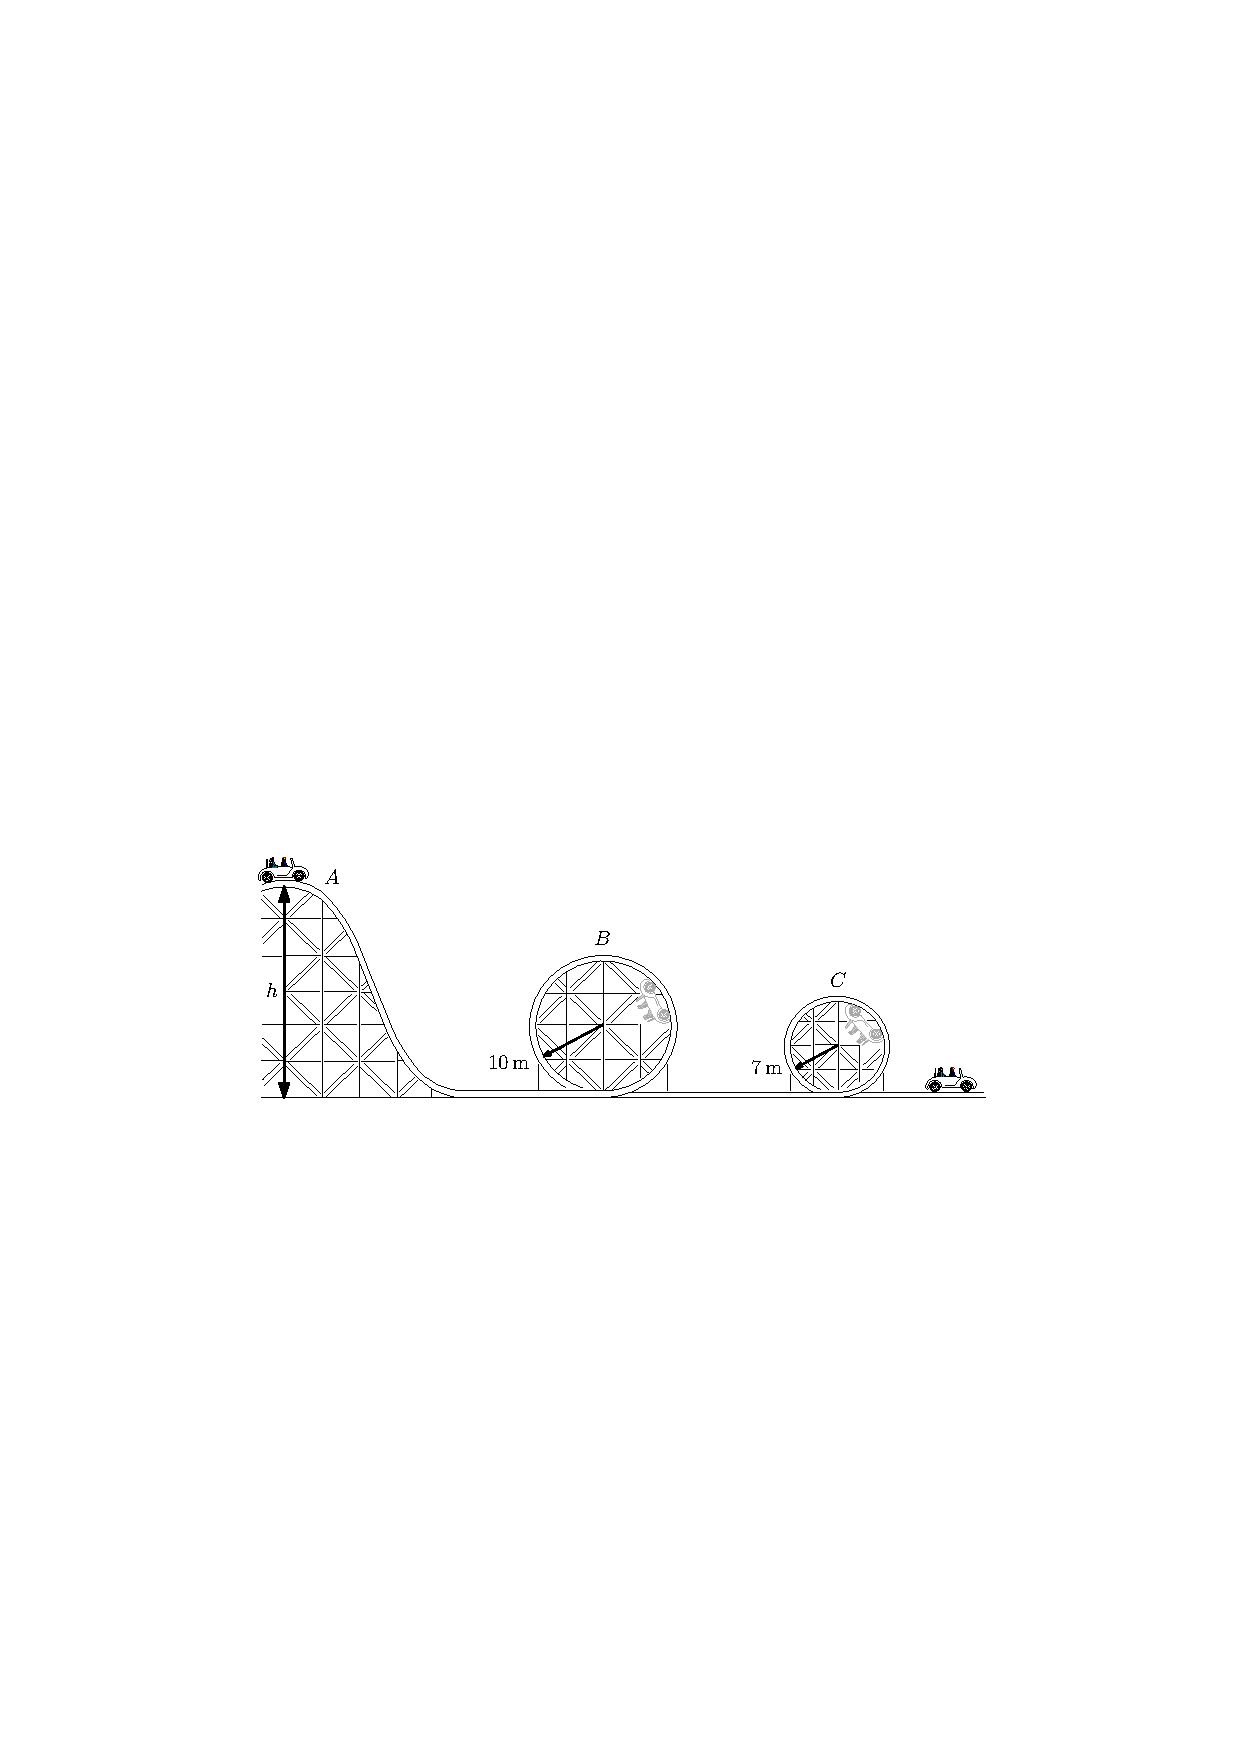
\includegraphics[scale=1.3]{images/draw_15.pdf}
\end{flushleft}